\chapter{Конструкторская часть}

\section{Требования к программному обеспечению}

\begin{enumerate}
  \item программа запрашивает размер массива $N$~--- натуральное число;
  \item программа формирует массив из $N$ различных целых чисел;
  \item программа создаёт копию исходного массива и сортирует её
    по возрастанию, исходный массив не изменяется;
  \item программа циклически выводит меню со следующими пунктами:
    \begin{itemize}
      \item выбранный алгоритм;
      \item поиск элемента текущим алгоритмом;
      \item поиск элемента всеми алгоритмами;
      \item выбор алгоритма;
      \item вывод массива;
      \item выполнение тестов;
      \item завершение работы.
    \end{itemize}
\end{enumerate}

\section{Разработка алгоритмов}
%2) разработать рекурсивный и нерекурсивные алгоритмы решения задачи, согласно варианту;
Для каждого алгоритма определены:
\begin{itemize}
	\item $array$~--- входной массив;
	\item $N$~--- количество элементов в $array$;
	\item $t$~--- искомый элемент;
	\item $index$~--- индекс искомого элемента.
\end{itemize}

Для алгоритмов бинарного поиска определены:
\begin{itemize}
	\item $l$~--- индекс левой границы;
	\item $r$~--- индекс правой границы;
	\item $m$~--- индекс рассматриваемого элемента.
\end{itemize}

\subsection{Поиск полным перебором}
При поиске полным перебором рассматривается каждый элемент массива и сравнивается с искомым. Если рассматриваемый элемент совпадает с искомым, его индекс запоминается и считается результатом поиска, после чего перебор прекращается. Временная сложность алгоритма~--- $O(N)$~\cite[с.~28]{laaksonen2024}.

Схема алгоритма поиска полным перебором приведена на рисунке~\ref{img:algo-brute-force}.

\begin{figure}[H]
	\centering
	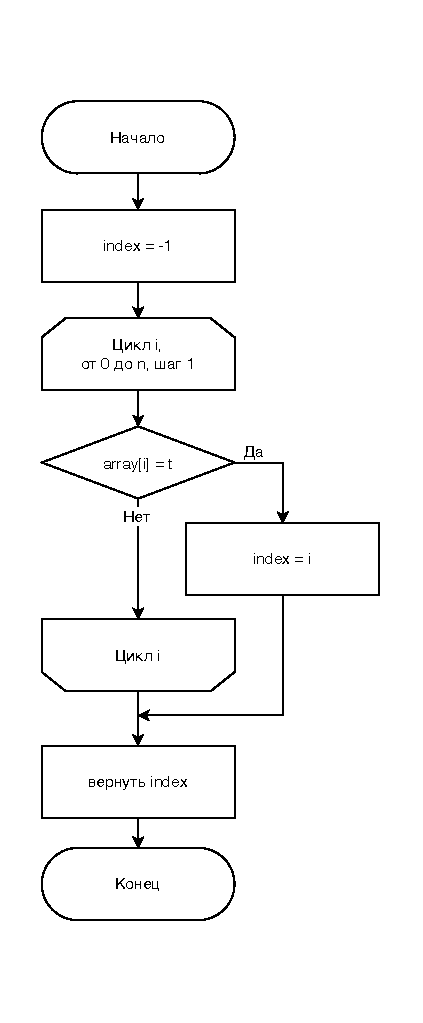
\includegraphics{image/algo/algo-brute-force.pdf}
	\caption{Схема алгоритма поиска полным перебором}
	\label{img:algo-brute-force}
\end{figure}

\subsection{Бинарный поиск}
Бинарный поиск применяется к массиву, отсортированному по возрастанию~\cite[с.~53]{laaksonen2024}. Изначально $l = 0$, $r = N - 1$. На каждой итерации поиска определяется средний элемент массива с индексом

\begin{equation}
	\label{eq:bin_s_m}
	m = l + \left\lfloor \frac{r - l}{2} \right\rfloor
\end{equation}

Для следующей итерации определяются новые границы массива
\begin{equation}
	\label{eq:new_l}
	l = 
	\begin{cases}
		m+1 & \text{array[m] < t} \\
		l & \text{иначе}
	\end{cases}
\end{equation}
\begin{equation}
	\label{eq:new_r}
	r = 
	\begin{cases}
		m & \text{array[m]} \geq \text{t} \\
		r & \text{иначе}
	\end{cases}
\end{equation}
Поиск продолжается до тех пор, пока $l < r$. После завершения цикла элемент $array[l]$ сравнивается с искомым: при совпадении результатом поиска является индекс $l$, иначе искомый элемент в массиве отсутствует.

Уменьшение размера массива в два раза на каждой итерации позволяет добиться временной сложности $O(\log{N})$~\cite[с.~53]{laaksonen2024}, но при этом требуется, чтобы массив поступал и поддерживался отсортированным.


%3) описать разработанные алгоритмы схемами алгоритмов;
%\section{Схемы алгоритмов}

% Схемы выгружаются из algo.drawio в img/algo/*.pdf скриптом export-algo.sh
Схемы нерекурсивных алгоритмов бинарного поиска приведены на рисунках~\ref{img:algo-bin-search-1} и~\ref{img:algo-bin-search-2}.

\begin{figure}[H]
	\centering
	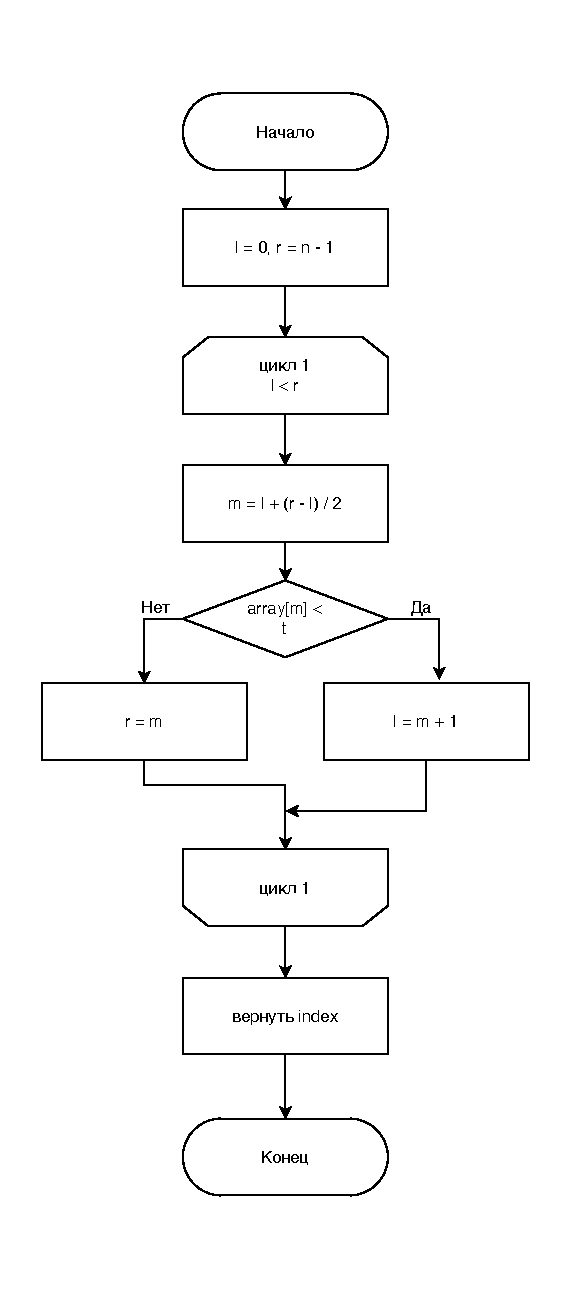
\includegraphics{image/algo/algo-bin-search-1.pdf}
	\caption{Схема нерекурсивного алгоритма бинарного поиска}
	\label{img:algo-bin-search-1}
\end{figure}


\begin{figure}[H]
	\centering
	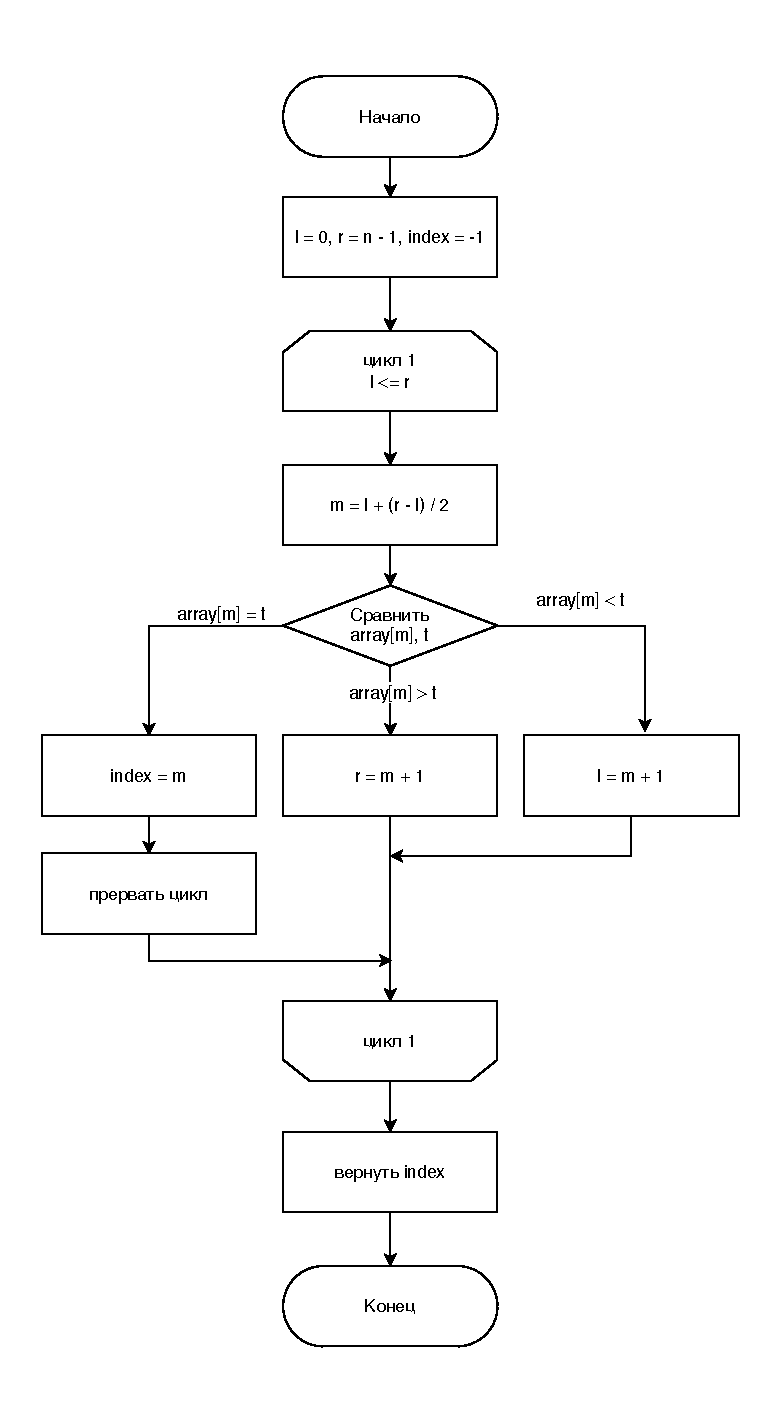
\includegraphics{image/algo/algo-bin-search-2.pdf}
	\caption{Схема нерекурсивного алгоритма бинарного поиска с предварительным выходом}
	\label{img:algo-bin-search-2}
\end{figure}

Схема рекурсивного алгоритма бинарного поиска приведена на рисунке~\ref{img:algo-bin-search-r}.

\begin{figure}[H]
	\centering
	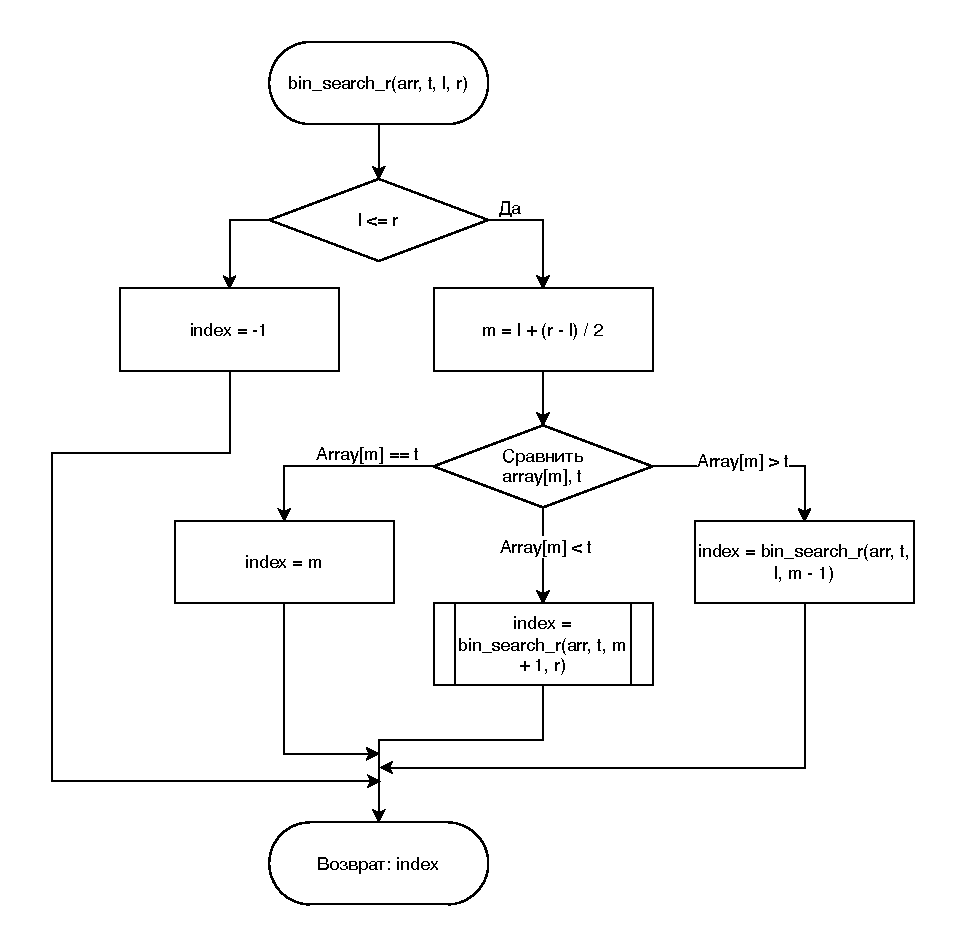
\includegraphics{image/algo/algo-bin-search-r.pdf}
	\caption{Схема рекурсивного алгоритма бинарного поиска}
	\label{img:algo-bin-search-r}
\end{figure}

\section{Вывод}
В результате конструкторской части были определены требования к программному обеспечению, спроектированы алгоритм полного перебора, два варианта алгоритма нерекурсивного бинарного поиска и алгоритм рекурсивного бинарного поиска.


%4) описать требования к программному обеспечению; // см. семинар 1
